\documentclass[twoside, a3paper]{report}
\usepackage[utf8]{inputenc}
\usepackage[T2A]{fontenc}
\usepackage{graphicx}
\usepackage{geometry}
\usepackage{lipsum}
\usepackage{amsmath, amsthm, amsfonts, amssymb}
\usepackage{tikz, pgfplots}
\usetikzlibrary{calc}
\usetikzlibrary{positioning}
\usetikzlibrary{shapes.geometric}
\usetikzlibrary{arrows.meta}
\usepackage{titlesec}
\usepackage{listings}
\usepackage{xcolor}
\usepackage{etoolbox}
\usepackage{lipsum}
\usepackage{latexsym}
%\usepackage[OT1]{fontenc}
\usepgflibrary{shadings}
\usetikzlibrary{shadings}
\pgfplotsset{compat=newest} % Важно для корректной работы современных функций








\lstloadlanguages{C,C++,csh,Java}

%\definecolor{red}{rgb}{0.6,0,0} 
%\definecolor{blue}{rgb}{0,0,0.6}
%\definecolor{green}{rgb}{0,0.8,0}
%\definecolor{cyan}{rgb}{0.0,0.6,0.6}

\lstset{
	language=csh,
	basicstyle=\footnotesize\ttfamily,
	numbers=left,
	numberstyle=\tiny,
	numbersep=5pt,
	tabsize=2,
	extendedchars=true,
	breaklines=true,
	frame=b,
	stringstyle=\color{blue}\ttfamily,
	showspaces=false,
	showtabs=false,
	xleftmargin=17pt,
	framexleftmargin=17pt,
	framexrightmargin=5pt,
	framexbottommargin=4pt,
	commentstyle=\color{green},
	morecomment=[l]{//}, %use comment-line-style!
	morecomment=[s]{/*}{*/}, %for multiline comments
	showstringspaces=false,
	morekeywords={ abstract, event, new, struct,
		as, explicit, null, switch,
		base, extern, object, this,
		bool, false, operator, throw,
		break, finally, out, true,
		byte, fixed, override, try,
		case, float, params, typeof,
		catch, for, private, uint,
		char, foreach, protected, ulong,
		checked, goto, public, unchecked,
		class, if, readonly, unsafe,
		const, implicit, ref, ushort,
		continue, in, return, using,
		decimal, int, sbyte, virtual,
		default, interface, sealed, volatile,
		delegate, internal, short, void,
		do, is, sizeof, while,
		double, lock, stackalloc,
		else, long, static,
		enum, namespace, string},
	keywordstyle=\color{blue},
	identifierstyle=\color{black},
	stringstyle=\color{red},
	backgroundcolor=\color{white},
}

\usepackage{caption}
\DeclareCaptionFont{white}{\color{white}}
\DeclareCaptionFormat{listing}{\colorbox{blue}{\parbox{\textwidth}{\hspace{15pt}#1#2#3}}}
\captionsetup[lstlisting]{format=listing,labelfont=white,textfont=white, singlelinecheck=false, margin=0pt, font={bf,footnotesize}}

\newtoggle{InString}{}% Keep track of if we are within a string
\togglefalse{InString}% Assume not initally in string

\newcommand*{\ColorIfNotInString}[1]{\iftoggle{InString}{#1}{\color{red}#1}}%
\newcommand*{\ProcessQuote}[1]{#1\iftoggle{InString}{\global\togglefalse{InString}}{\global\toggletrue{InString}}}%
\lstset{literate=%
	{"}{{{\ProcessQuote{"}}}}1% Disable coloring within double quotes
	{'}{{{\ProcessQuote{'}}}}1% Disable coloring within single quote
	{0}{{{\ColorIfNotInString{0}}}}1
	{1}{{{\ColorIfNotInString{1}}}}1
	{2}{{{\ColorIfNotInString{2}}}}1
	{3}{{{\ColorIfNotInString{3}}}}1
	{4}{{{\ColorIfNotInString{4}}}}1
	{5}{{{\ColorIfNotInString{5}}}}1
	{6}{{{\ColorIfNotInString{6}}}}1
	{7}{{{\ColorIfNotInString{7}}}}1
	{8}{{{\ColorIfNotInString{8}}}}1
	{9}{{{\ColorIfNotInString{9}}}}1
}


\newgeometry{
	top    = 15pt,
	bottom = 40pt,
	outer  = 25pt,
	inner  = 80pt,
}


































\begin{document}



\chapter{Заметки}

рассмотрим следующую задачу: у нас есть некоторое количество входов, с произвольным входом. Требуется перераспределить их между тем же количеством выходов, так, чтобы на каждом из них был одинаковый поток.

\

Очевидно, для \underline{произвольного} значения входа, решение единственно:


\vspace{0.5in}

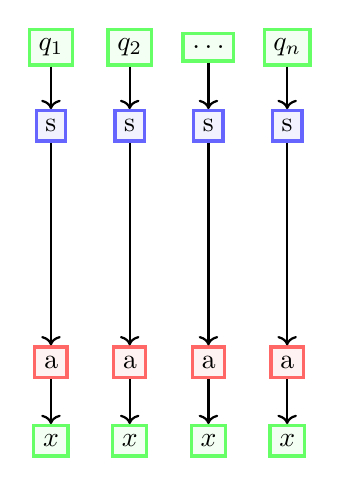
\begin{tikzpicture}[
	s/.style = {rectangle, draw=blue!60,	fill=blue!5,	very thick, minimum size=10},
	a/.style = {rectangle, draw=red!60,		fill=red!5,		very thick, minimum size=10},
	o/.style = {rectangle, draw=green!60,	fill=green!5,	very thick, minimum size=10},
	r/.style = {->, thick, rounded corners=5pt}
	]
	
	
	% === === Nodes === ===
	\node[o]	(in1)	at	(-2, 2)		{$q_1$};
	\node[o]	(in2)	at	(-1, 2)		{$q_2$};
	\node[o]	(ine)	at	(0, 2)		{$\ldots$};
	\node[o]	(inn)	at	(1, 2)		{$q_n$};
	
	\node[s]	(s1)	at	(-2, 1)		{s};
	\node[s]	(s2)	at	(-1, 1)		{s};
	\node[s]	(se)	at	(0, 1)		{s};
	\node[s]	(sn)	at	(1, 1)		{s};
	
	\node[a]	(a1)	at	(-2, -2)	{a};
	\node[a]	(a2)	at	(-1, -2)	{a};
	\node[a]	(ae)	at	(0, -2)		{a};
	\node[a]	(an)	at	(1, -2)		{a};
	
	\node[o]	(out1)	at	(-2, -3)	{$x$};
	\node[o]	(out2)	at	(-1, -3)	{$x$};
	\node[o]	(oute)	at	(0, -3)		{$x$};
	\node[o]	(outn)	at	(1, -3)		{$x$};
	
	
	
	% === === Lines === ===
	\draw[r]	(in1.south)	to	(s1.north);
	\draw[r]	(in2.south)	to	(s2.north);
	\draw[r]	(ine.south)	to	(se.north);
	\draw[r]	(inn.south)	to	(sn.north);
	
	\draw[r]	(a1.south)	to	(out1.north);
	\draw[r]	(a2.south)	to	(out2.north);
	\draw[r]	(ae.south)	to	(oute.north);
	\draw[r]	(an.south)	to	(outn.north);
	
	\draw[r]	(s1.south)	to	(a1.north);
	\draw[r]	(s2.south)	to	(a2.north);
	\draw[r]	(se.south)	to	(ae.north);
	\draw[r]	(sn.south)	to	(an.north);
	
	
\end{tikzpicture}
















\newpage
\thispagestyle{empty}
\mbox{}
\newpage

Входы: 4, 8, 10, 18

Выходы: 5, 8, 12, 15

\

$$
\left[
\begin{matrix}
	5 \\ 8 \\ 15 \\ 12
\end{matrix}
\right]
=
\left[
\begin{matrix}
	\frac12 & 0 & 0 & 0 \\
	0 		& 1 & 0 & 0 \\
	\frac12 & 0 & 1	& \frac13 \\
	0		& 0 & 0 & \frac23 \\
\end{matrix}
\right]
\times
\left[
\begin{matrix}
	10 \\ 8 \\ 4 \\ 18
\end{matrix}
\right]
$$

\

$$
\left[
\begin{matrix}
	10 \\ 8 \\ 4 \\ 18
\end{matrix}
\right]
=
\left[
\begin{matrix}
	1 & 0 & \frac13 & 0 \\
	0 & 1 & 0       & 0 \\
	0 & 0 & \frac23	& \frac13 \\
	0 & 0 & 0       & \frac23 \\
\end{matrix}
\right]
\times
\left[
\begin{matrix}
	5 \\ 8 \\ 15 \\ 12
\end{matrix}
\right]
$$

\

$$
\left[
\begin{matrix}
	\frac12 & 0 & \frac16 & 0 \\
	0 		& 1 & 0       & 0 \\
	\frac12 & 0 & \frac16 & \frac23 \\
	0		& 0 & \frac13 & \frac13 \\
\end{matrix}
\right] \ \equiv \ \left[
\begin{matrix}
	\frac23 & 0 & \frac13 & \frac16 \\
	0 		& 1 & 0       & 0 \\
	0       & 0 & 0       & \frac16 \\
	\frac13	& 0 & \frac23 & \frac13 \\
\end{matrix}
\right] \ \equiv \ \left[
\begin{matrix}
	1 & 0 & 0 & 0 \\
	0 & 1 & 0 & 0 \\
	0 & 0 & 1 & 0 \\
	0 & 0 & 0 & 1 \\
\end{matrix}
\right]
$$





\vspace{0.5in}

$$
\left[
\begin{matrix}
	\alpha\beta + \frac{b-\alpha}{a} - \beta \cdot \frac{b-\alpha}{a} & 
	\alpha \cdot \frac{1-\beta b}{1+a-b} + \frac{b-\alpha}{a} - \frac{b-\alpha}{a} \cdot \frac{1-\beta b}{1 + a - b} \\
	1 - \alpha\beta - \frac{b-\alpha}{a} + \beta \cdot \frac{b-\alpha}{a} & 
	1 - \alpha \cdot \frac{1-\beta b}{1+a-b} - \frac{b-\alpha}{a} + \frac{b-\alpha}{a} \cdot \frac{1-\beta b}{1 + a - b}
\end{matrix}
\right]
\ \equiv \
$$

$$
\ \equiv \
\left[
\begin{matrix}
	\alpha\beta + \frac{1-\beta b}{1 + a - b} - \alpha \cdot \frac{1-\beta b}{1 + a - b} & 
	\beta \cdot \frac{b-\alpha}{a} + \frac{1-\beta b}{1+a-b} - \frac{b-\alpha}{a} \cdot \frac{1 - \beta b}{1 + a - b} \\
	1 - \alpha\beta - \frac{1-\beta b}{1 + a - b} + \alpha \cdot \frac{1-\beta b}{1 + a - b} & 
	1 - \beta \cdot \frac{b-\alpha}{a} - \frac{1-\beta b}{1+a-b} + \frac{b-\alpha}{a} \cdot \frac{1 - \beta b}{1 + a - b}
\end{matrix}
\right]
\ \equiv \
$$

$$
\ \equiv \
\left[
\begin{matrix}
	1 & 0 \\
	0 & 1
\end{matrix}
\right]
$$


















\newpage

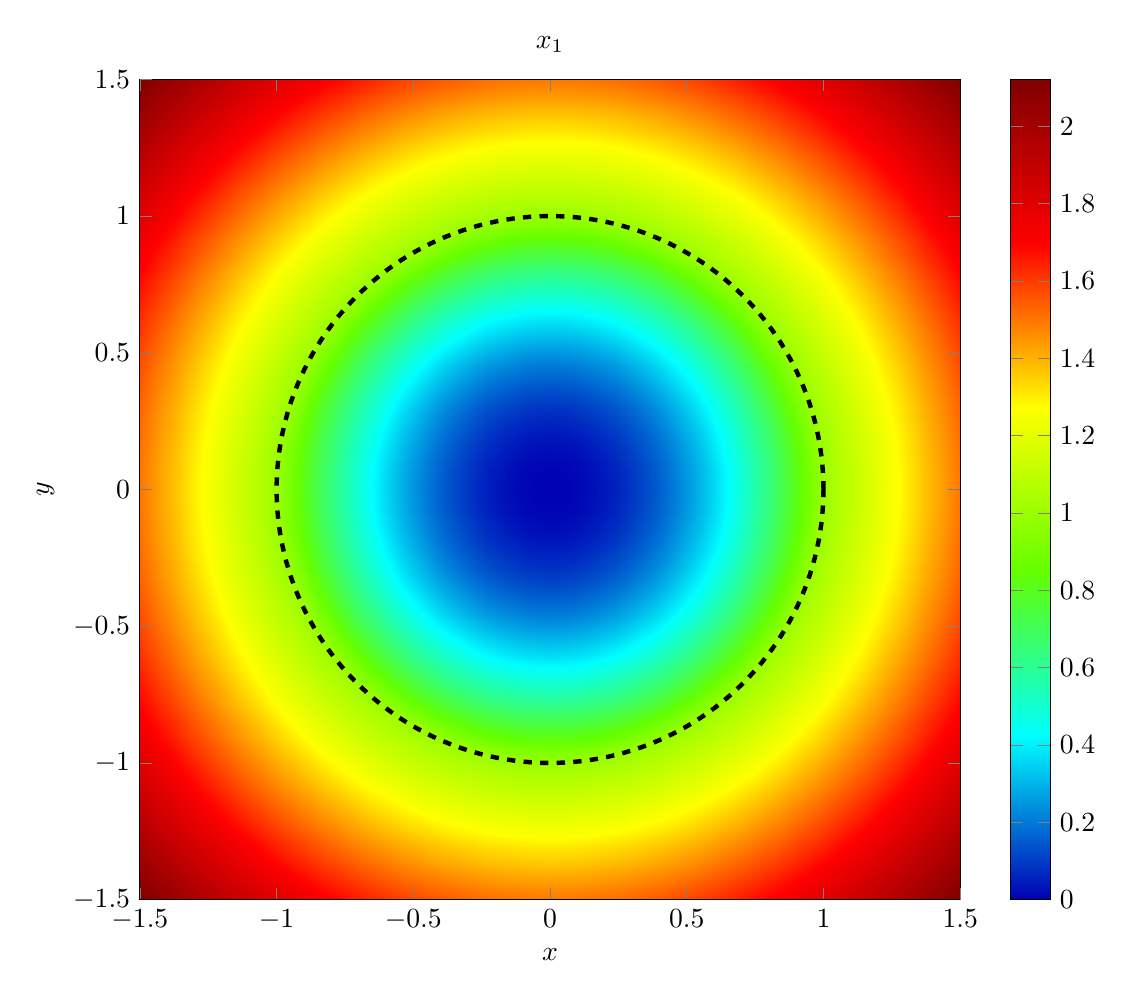
\begin{tikzpicture}
	\begin{axis}[
		width=12cm,
		height=12cm,
		axis equal image, % Сохраняет пропорции круга
		view={0}{90},     % Вид строго сверху (проецирует 3D-поверхность на плоскость)
		colorbar,         % Добавляет легенду цветов
		colormap/bluered, % Стандартная палитра: синий (минимум) -> красный (максимум)
		xlabel=$x$, ylabel=$y$,
		title={$x_1$},
		enlargelimits=false, % Не добавляет отступы за пределы области определения
		]
		
		\addplot3[
			surf,
			shader=interp,
			domain=-1.5:1.5,
			domain y=-1.5:1.5,
			samples=81,
			samples y=81,
			point meta=z
			] (x, y, {(x^2 + y^2 <= 1) ? (x^2 + y^2) : (sqrt(x^2+y^2))});
		
		\draw[ultra thick, black, dashed]  plot[domain=0:360, samples=200] ({cos(\x)}, {sin(\x)});
		
	\end{axis}
\end{tikzpicture}







\newpage

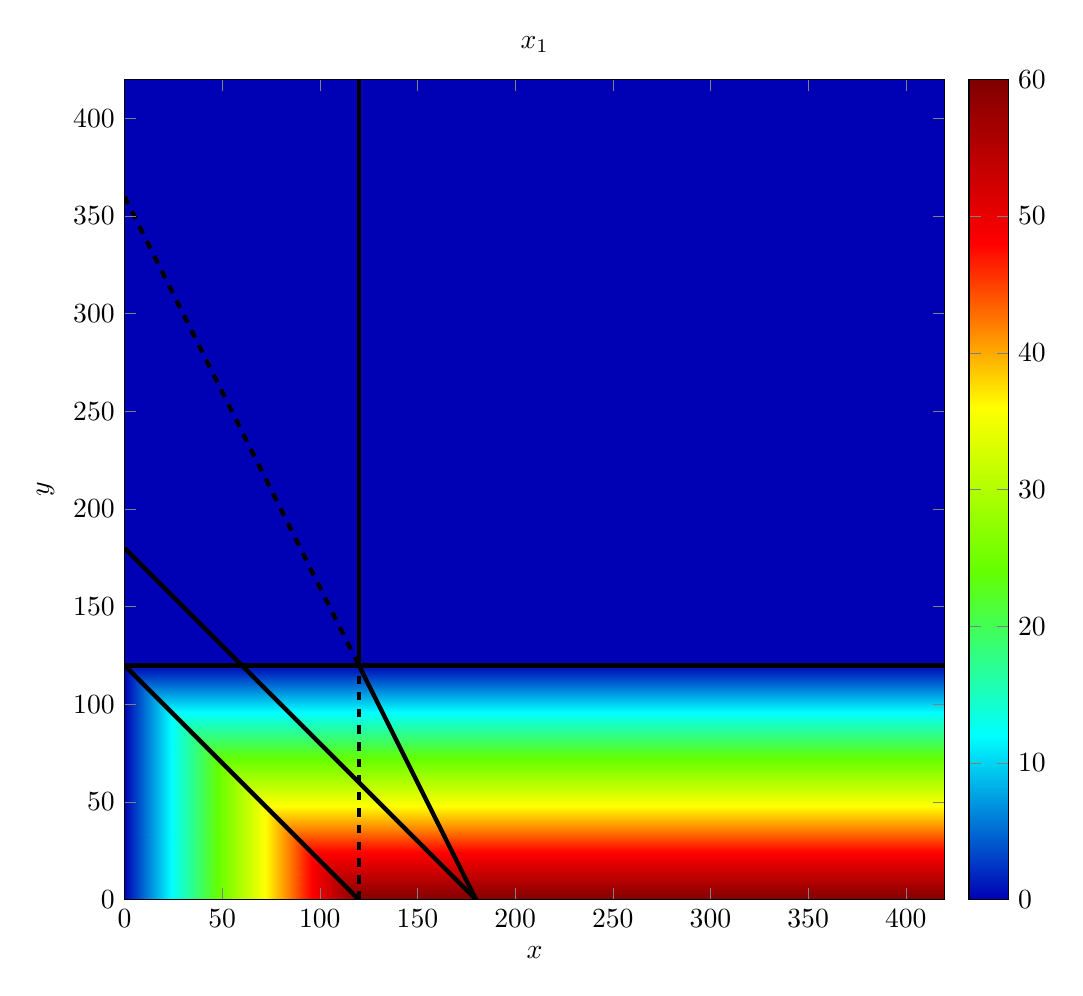
\begin{tikzpicture}
	\begin{axis}[
		width=12cm,
		height=12cm,
		axis equal image, % Сохраняет пропорции круга
		view={0}{90},     % Вид строго сверху (проецирует 3D-поверхность на плоскость)
		colorbar,         % Добавляет легенду цветов
		colormap/bluered, % Стандартная палитра: синий (минимум) -> красный (максимум)
		xlabel=$x$, ylabel=$y$,
		title={$x_1$},
		enlargelimits=false, % Не добавляет отступы за пределы области определения
		]
		
		% Основная команда отрисовки
		\addplot3[
		surf,          % Режим заливки цветом по значению z
		shader=interp, % Плавные переходы между цветами (интерполяция)
		domain=0:420, % Область по x
		domain y=0:420, % Область по y
		samples=84,   % Количество точек сетки (чем больше, тем плавнее круг)
		samples y=84,
		point meta=z   % Цвет берется из значения координаты z
		] (x, y, {
			(y <= 120) 
			? (
				(x+y <= 120) 
				? (x/2) 
				: (60-y/2)
			) 
			: (0)
			});
		
		
		
		\draw[ultra thick, black] 			plot[domain=0:120, samples=84]		({\x}, {120-\x});
		\draw[ultra thick, black] 			plot[domain=0:180, samples=84]		({\x}, {180-\x});
		\draw[ultra thick, black] 			plot[domain=120:180, samples=84]	({\x}, {360-2*\x});
		\draw[ultra thick, black, dashed]	plot[domain=0:120, samples=84]		({\x}, {360-2*\x});
		\draw[ultra thick, black] 			plot[domain=0:420, samples=84]		({\x}, {120});
		\draw[ultra thick, black] 			plot[domain=120:420, samples=84]	({120}, {\x});
		\draw[ultra thick, black, dashed] 	plot[domain=00:120, samples=84]		({120}, {\x});
		
	\end{axis}
\end{tikzpicture}





\vspace{0.5in}

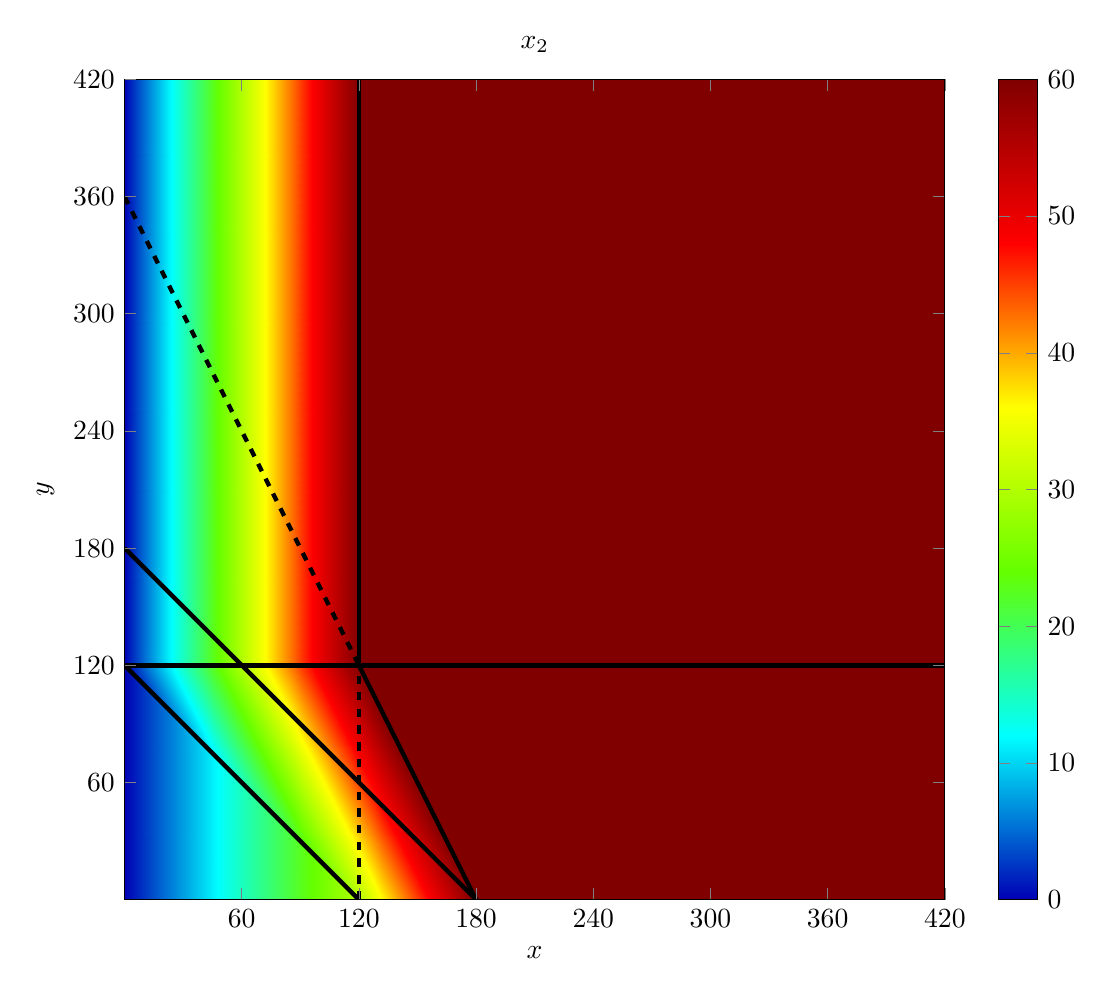
\begin{tikzpicture}
	\begin{axis}[
		width=12cm,
		height=12cm,
		axis equal image, % Сохраняет пропорции круга
		view={0}{90},     % Вид строго сверху (проецирует 3D-поверхность на плоскость)
		colorbar,         % Добавляет легенду цветов
		colormap/bluered, % Стандартная палитра: синий (минимум) -> красный (максимум)
		xlabel=$x$, ylabel=$y$,
		title={$x_2$},
		enlargelimits=false, % Не добавляет отступы за пределы области определения
		xtick = {60, 120, 180, 240, 300, 360, 420}, 
		xticklabels = {$60$, $120$, $180$, $240$, $300$, $360$, $420$},
		ytick = {60, 120, 180, 240, 300, 360, 420}, 
		yticklabels = {$60$, $120$, $180$, $240$, $300$, $360$, $420$},
		]
		
		% Основная команда отрисовки
		\addplot3[
		surf,          % Режим заливки цветом по значению z
		shader=interp, % Плавные переходы между цветами (интерполяция)
		domain=0:420, % Область по x
		domain y=0:420, % Область по y
		samples=84,   % Количество точек сетки (чем больше, тем плавнее круг)
		samples y=84,
		point meta=z   % Цвет берется из значения координаты z
		] (x, y, {
			(y <= 120) 
			? (
			(x+y <= 120) 
			? (x/4) % 0
			: (
			(x+y <= 180) 
			? (x/2+y/4-30) % 1
			: (
			(2*x+y <= 360) 
			? (x/2+y/4-30) % 2 
			: (60) % 3
			)
			)
			) 
			: (
			(x+y <= 180) 
			? (x/2) % 4
			: (
			(x <= 120) 
			? (x/2)  % 5
			: (60) % 6
			)
			)
		});
		
		
		
		\draw[ultra thick, black] 			plot[domain=0:120, samples=84]		({\x}, {120-\x});
		\draw[ultra thick, black] 			plot[domain=0:180, samples=84]		({\x}, {180-\x});
		\draw[ultra thick, black] 			plot[domain=120:180, samples=84]	({\x}, {360-2*\x});
		\draw[ultra thick, black, dashed]	plot[domain=0:120, samples=84]		({\x}, {360-2*\x});
		\draw[ultra thick, black] 			plot[domain=0:420, samples=84]		({\x}, {120});
		\draw[ultra thick, black] 			plot[domain=120:420, samples=84]	({120}, {\x});
		\draw[ultra thick, black, dashed] 	plot[domain=00:120, samples=84]		({120}, {\x});
		
	\end{axis}
\end{tikzpicture}










\vspace{0.5in}

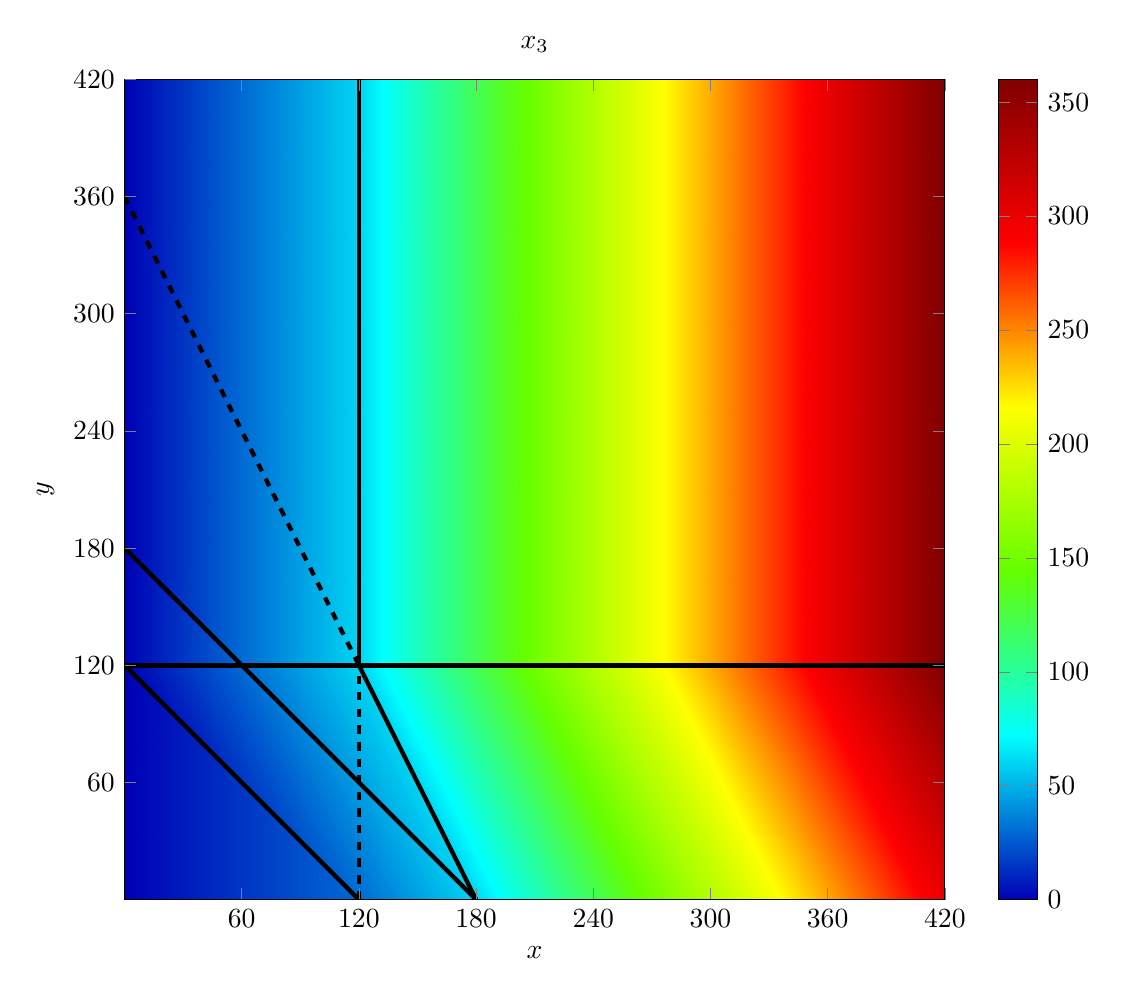
\begin{tikzpicture}
	\begin{axis}[
		width=12cm,
		height=12cm,
		axis equal image, % Сохраняет пропорции круга
		view={0}{90},     % Вид строго сверху (проецирует 3D-поверхность на плоскость)
		colorbar,         % Добавляет легенду цветов
		colormap/bluered, % Стандартная палитра: синий (минимум) -> красный (максимум)
		xlabel=$x$, ylabel=$y$,
		title={$x_3$},
		enlargelimits=false, % Не добавляет отступы за пределы области определения
		xtick = {60, 120, 180, 240, 300, 360, 420}, 
		xticklabels = {$60$, $120$, $180$, $240$, $300$, $360$, $420$},
		ytick = {60, 120, 180, 240, 300, 360, 420}, 
		yticklabels = {$60$, $120$, $180$, $240$, $300$, $360$, $420$},
		]
		
		% Основная команда отрисовки
		\addplot3[
		surf,          % Режим заливки цветом по значению z
		shader=interp, % Плавные переходы между цветами (интерполяция)
		domain=0:420, % Область по x
		domain y=0:420, % Область по y
		samples=84,   % Количество точек сетки (чем больше, тем плавнее круг)
		samples y=84,
		point meta=z   % Цвет берется из значения координаты z
		] (x, y, {
			(y <= 120) 
			? (
			(x+y <= 120) 
			? (x/4) % 0
			: (
			(x+y <= 180) 
			? (x/2+y/4-30) % 1
			: (
			(2*x+y <= 360) 
			? (x/2+y/4-30) % 2 
			: (x+y/2-120) % 3
			)
			)
			) 
			: (
			(x+y <= 180) 
			? (x/2) % 4
			: (
			(x <= 120) 
			? (x/2)  % 5
			: (x-60) % 6
			)
			)
		});
		
		
		
		\draw[ultra thick, black] 			plot[domain=0:120, samples=84]		({\x}, {120-\x});
		\draw[ultra thick, black] 			plot[domain=0:180, samples=84]		({\x}, {180-\x});
		\draw[ultra thick, black] 			plot[domain=120:180, samples=84]	({\x}, {360-2*\x});
		\draw[ultra thick, black, dashed]	plot[domain=0:120, samples=84]		({\x}, {360-2*\x});
		\draw[ultra thick, black] 			plot[domain=0:420, samples=84]		({\x}, {120});
		\draw[ultra thick, black] 			plot[domain=120:420, samples=84]	({120}, {\x});
		\draw[ultra thick, black, dashed] 	plot[domain=00:120, samples=84]		({120}, {\x});
		
	\end{axis}
\end{tikzpicture}
























\newpage



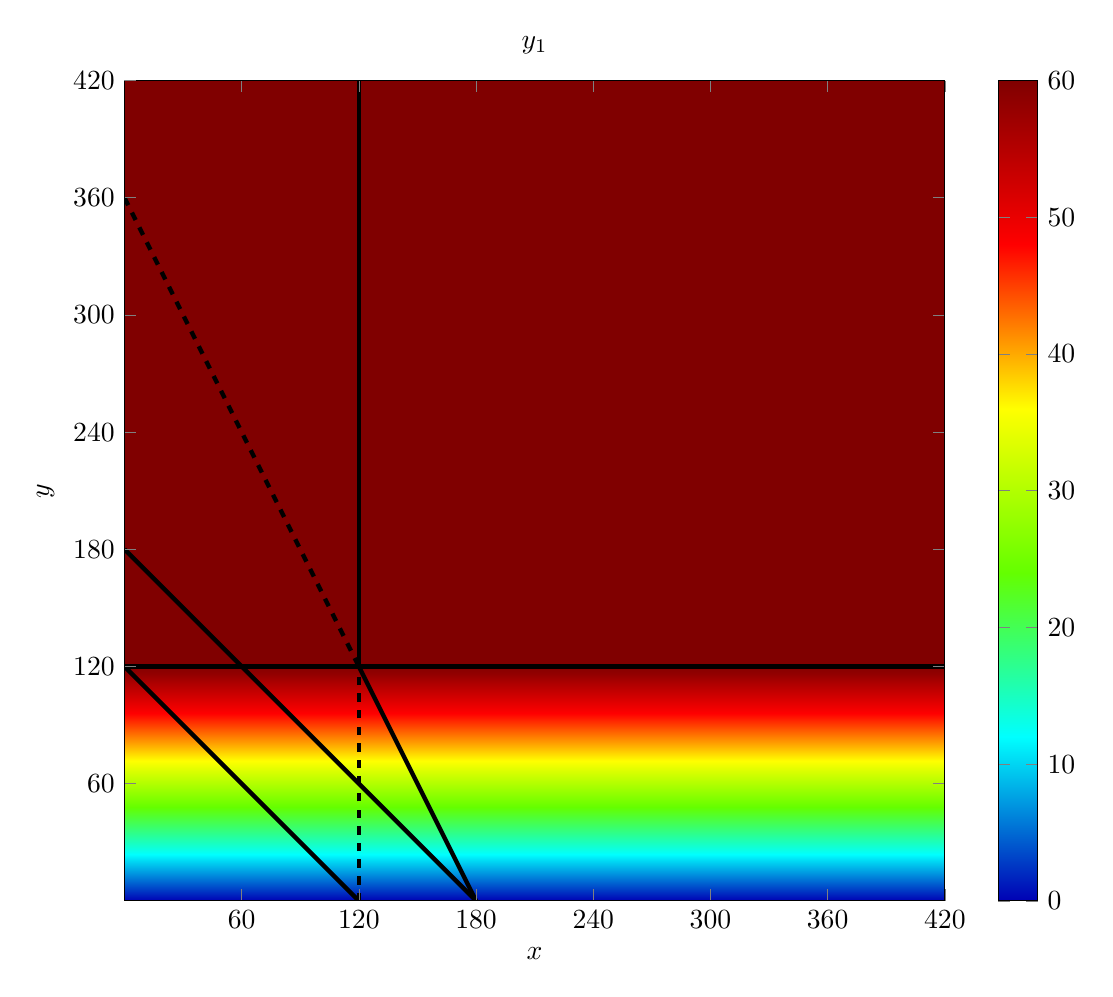
\begin{tikzpicture}
	\begin{axis}[
		width=12cm,
		height=12cm,
		axis equal image, % Сохраняет пропорции круга
		view={0}{90},     % Вид строго сверху (проецирует 3D-поверхность на плоскость)
		colorbar,         % Добавляет легенду цветов
		colormap/bluered, % Стандартная палитра: синий (минимум) -> красный (максимум)
		xlabel=$x$, ylabel=$y$,
		title={$y_1$},
		enlargelimits=false, % Не добавляет отступы за пределы области определения
		xtick = {60, 120, 180, 240, 300, 360, 420}, 
		xticklabels = {$60$, $120$, $180$, $240$, $300$, $360$, $420$},
		ytick = {60, 120, 180, 240, 300, 360, 420}, 
		yticklabels = {$60$, $120$, $180$, $240$, $300$, $360$, $420$},
		]
		
		% Основная команда отрисовки
		\addplot3[
		surf,          % Режим заливки цветом по значению z
		shader=interp, % Плавные переходы между цветами (интерполяция)
		domain=0:420, % Область по x
		domain y=0:420, % Область по y
		samples=84,   % Количество точек сетки (чем больше, тем плавнее круг)
		samples y=84,
		point meta=z   % Цвет берется из значения координаты z
		] (x, y, {
			(y <= 120) 
			? (
			(x+y <= 120) 
			? (y/2) % 0
			: (
			(x+y <= 180) 
			? (y/2) % 1
			: (
			(2*x+y <= 360) 
			? (y/2) % 2 
			: (y/2) % 3
			)
			)
			) 
			: (
			(x+y <= 180) 
			? (60) % 4
			: (
			(x <= 120) 
			? (60)  % 5
			: (60) % 6
			)
			)
		});
		
		
		
		\draw[ultra thick, black] 			plot[domain=0:120, samples=84]		({\x}, {120-\x});
		\draw[ultra thick, black] 			plot[domain=0:180, samples=84]		({\x}, {180-\x});
		\draw[ultra thick, black] 			plot[domain=120:180, samples=84]	({\x}, {360-2*\x});
		\draw[ultra thick, black, dashed]	plot[domain=0:120, samples=84]		({\x}, {360-2*\x});
		\draw[ultra thick, black] 			plot[domain=0:420, samples=84]		({\x}, {120});
		\draw[ultra thick, black] 			plot[domain=120:420, samples=84]	({120}, {\x});
		\draw[ultra thick, black, dashed] 	plot[domain=00:120, samples=84]		({120}, {\x});
		
	\end{axis}
\end{tikzpicture}









\vspace{0.5in}

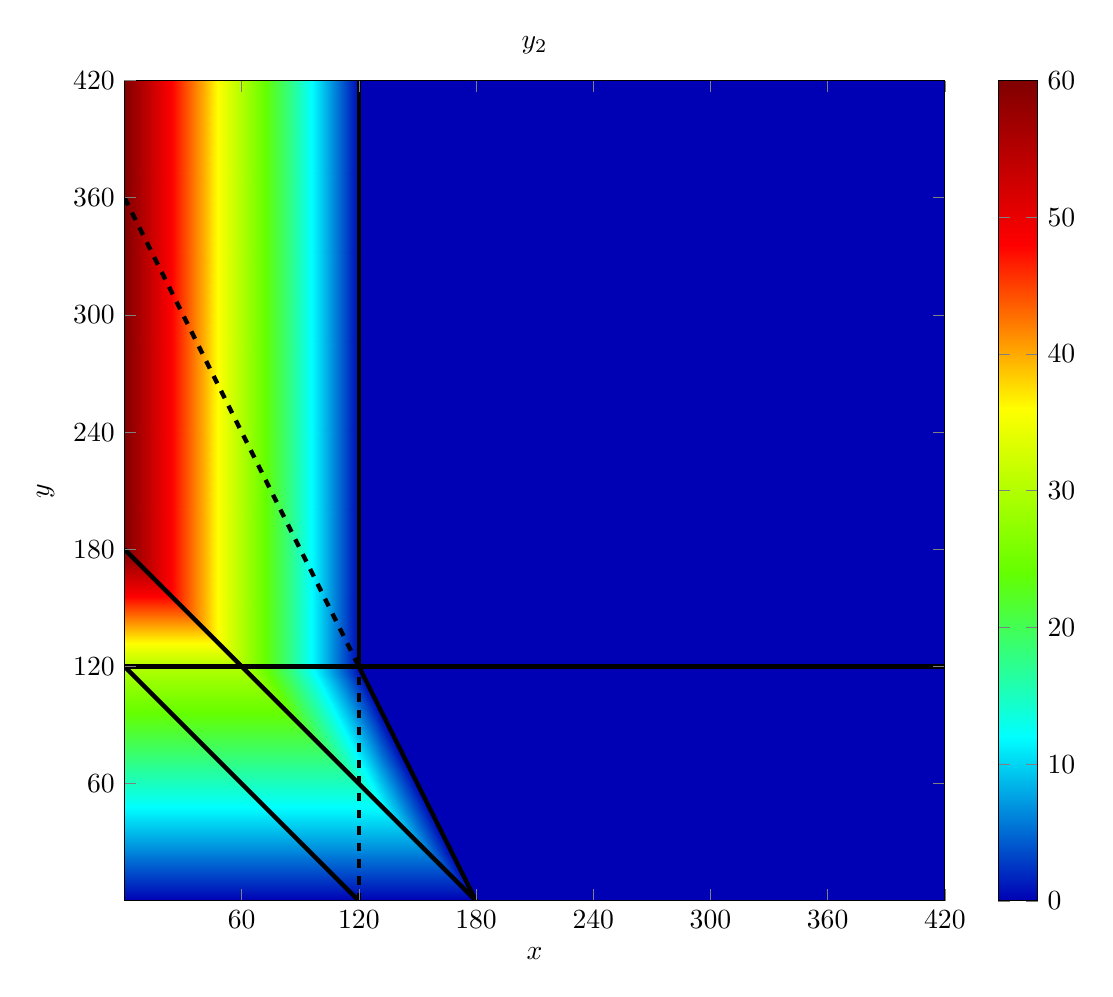
\begin{tikzpicture}
	\begin{axis}[
		width=12cm,
		height=12cm,
		axis equal image, % Сохраняет пропорции круга
		view={0}{90},     % Вид строго сверху (проецирует 3D-поверхность на плоскость)
		colorbar,         % Добавляет легенду цветов
		colormap/bluered, % Стандартная палитра: синий (минимум) -> красный (максимум)
		xlabel=$x$, ylabel=$y$,
		title={$y_2$},
		enlargelimits=false, % Не добавляет отступы за пределы области определения
		xtick = {60, 120, 180, 240, 300, 360, 420}, 
		xticklabels = {$60$, $120$, $180$, $240$, $300$, $360$, $420$},
		ytick = {60, 120, 180, 240, 300, 360, 420}, 
		yticklabels = {$60$, $120$, $180$, $240$, $300$, $360$, $420$},
		]
		
		% Основная команда отрисовки
		\addplot3[
		surf,          % Режим заливки цветом по значению z
		shader=interp, % Плавные переходы между цветами (интерполяция)
		domain=0:420, % Область по x
		domain y=0:420, % Область по y
		samples=84,   % Количество точек сетки (чем больше, тем плавнее круг)
		samples y=84,
		point meta=z   % Цвет берется из значения координаты z
		] (x, y, {
			(y <= 120) 
			? (
				(x+y <= 120) 
				? (y/4) % 0
				: (
					(x+y <= 180) 
					? (y/4) % 1
					: (
						(2*x+y <= 360) 
						? (90-x/2-y/4) % 2 
						: (0) % 3
					)
				)
			) 
			: (
				(x+y <= 180) 
				? (y/2-30) % 4
				: (
					(x <= 120) 
					? (60-x/2)  % 5
					: (0) % 6
				)
			)
		});
		
		
		
		\draw[ultra thick, black] 			plot[domain=0:120, samples=84]		({\x}, {120-\x});
		\draw[ultra thick, black] 			plot[domain=0:180, samples=84]		({\x}, {180-\x});
		\draw[ultra thick, black] 			plot[domain=120:180, samples=84]	({\x}, {360-2*\x});
		\draw[ultra thick, black, dashed]	plot[domain=0:120, samples=84]		({\x}, {360-2*\x});
		\draw[ultra thick, black] 			plot[domain=0:420, samples=84]		({\x}, {120});
		\draw[ultra thick, black] 			plot[domain=120:420, samples=84]	({120}, {\x});
		\draw[ultra thick, black, dashed] 	plot[domain=00:120, samples=84]		({120}, {\x});
		
	\end{axis}
\end{tikzpicture}












\vspace{0.5in}

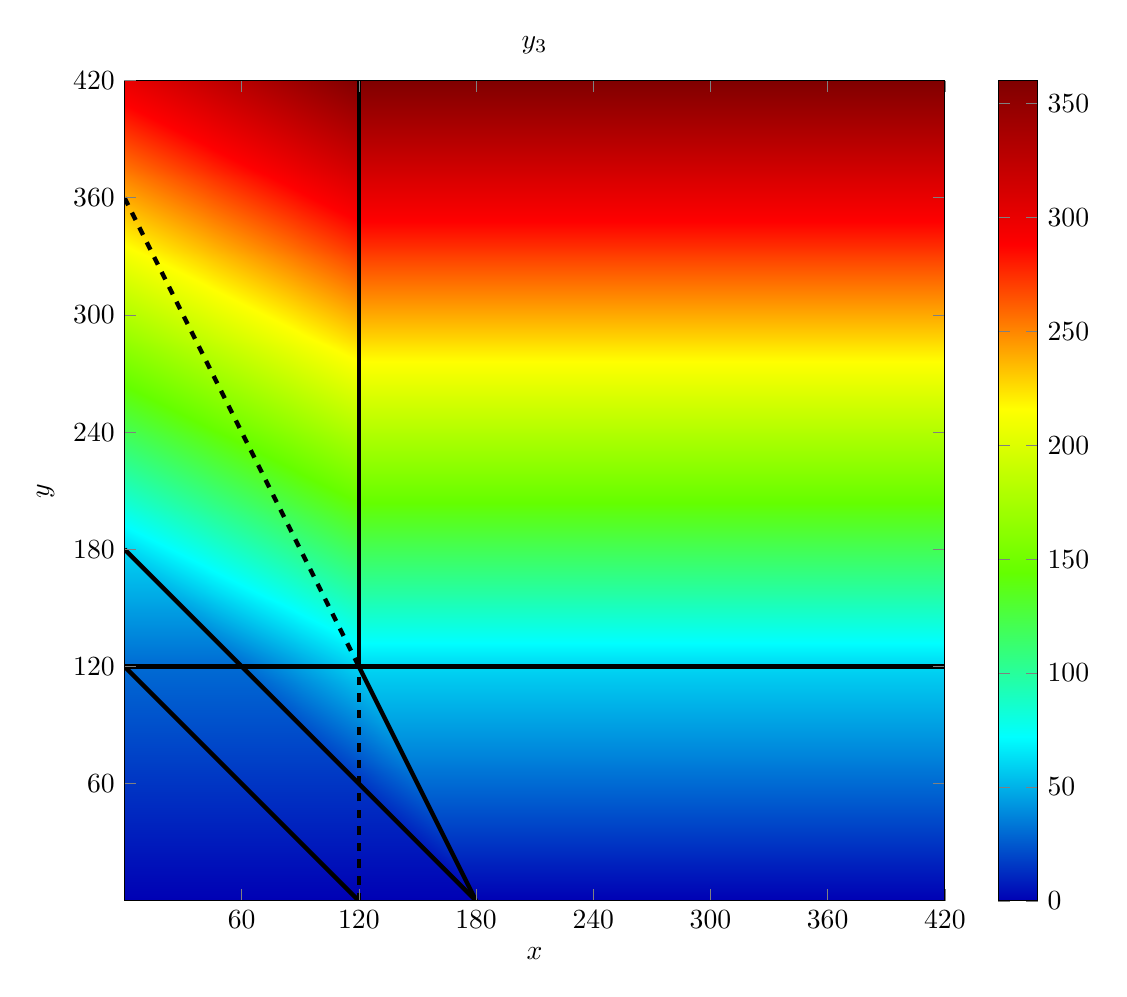
\begin{tikzpicture}
	\begin{axis}[
		width=12cm,
		height=12cm,
		axis equal image, % Сохраняет пропорции круга
		view={0}{90},     % Вид строго сверху (проецирует 3D-поверхность на плоскость)
		colorbar,         % Добавляет легенду цветов
		colormap/bluered, % Стандартная палитра: синий (минимум) -> красный (максимум)
		xlabel=$x$, ylabel=$y$,
		title={$y_3$},
		enlargelimits=false, % Не добавляет отступы за пределы области определения
		xtick = {60, 120, 180, 240, 300, 360, 420}, 
		xticklabels = {$60$, $120$, $180$, $240$, $300$, $360$, $420$},
		ytick = {60, 120, 180, 240, 300, 360, 420}, 
		yticklabels = {$60$, $120$, $180$, $240$, $300$, $360$, $420$},
		]
		
		% Основная команда отрисовки
		\addplot3[
		surf,          % Режим заливки цветом по значению z
		shader=interp, % Плавные переходы между цветами (интерполяция)
		domain=0:420, % Область по x
		domain y=0:420, % Область по y
		samples=84,   % Количество точек сетки (чем больше, тем плавнее круг)
		samples y=84,
		point meta=z   % Цвет берется из значения координаты z
		] (x, y, {
			(y <= 120) 
			? (
			(x+y <= 120) 
			? (y/4) % 0
			: (
			(x+y <= 180) 
			? (y/4) % 1
			: (
			(2*x+y <= 360) 
			? (x/2+3*y/4-90) % 2 
			: (y/2) % 3
			)
			)
			) 
			: (
			(x+y <= 180) 
			? (y/2-30) % 4
			: (
			(x <= 120) 
			? (x/2+y-120)  % 5
			: (y-60) % 6
			)
			)
		});
		
		
		
		\draw[ultra thick, black] 			plot[domain=0:120, samples=84]		({\x}, {120-\x});
		\draw[ultra thick, black] 			plot[domain=0:180, samples=84]		({\x}, {180-\x});
		\draw[ultra thick, black] 			plot[domain=120:180, samples=84]	({\x}, {360-2*\x});
		\draw[ultra thick, black, dashed]	plot[domain=0:120, samples=84]		({\x}, {360-2*\x});
		\draw[ultra thick, black] 			plot[domain=0:420, samples=84]		({\x}, {120});
		\draw[ultra thick, black] 			plot[domain=120:420, samples=84]	({120}, {\x});
		\draw[ultra thick, black, dashed] 	plot[domain=00:120, samples=84]		({120}, {\x});
		
	\end{axis}
\end{tikzpicture}















\newpage
\begin{tabular}{|c||c|c|c||c|c|c|}
	\hline
	\textbackslash 
	&	$x_1$&			$x_2$&						$x_3$&						$y_1$&			$y_2$&						$y_3$ \\
	\hline
	\hline
	0&	$\frac{x}2$&	$\frac{x}4$&				$\frac{x}4$&				$\frac{y}2$&	$\frac{y}4$&				$\frac{y}4$	  \\
	\hline
	\hline
	1&	$60-\frac{y}2$&	$\frac{x}2+\frac{y}4-30$&	$\frac{x}2+\frac{y}4-30$&	$\frac{y}2$&	$\frac{y}4$&				$\frac{y}4$	  \\
	\hline
	2&	$60-\frac{y}2$&	$\frac{x}2+\frac{y}4-30$&	$\frac{x}2+\frac{y}4-30$&	$\frac{y}2$&	$90-\frac{x}2-\frac{y}4$&	$\frac{x}2+\frac{3y}4-90$	  \\
	\hline
	\hline
	3&	$60-\frac{y}2$&	$60$&						$x+\frac{y}2-120$&			$\frac{y}2$&	$0$&						$\frac{y}2$	  \\
	\hline
	\hline
	4&	$0$&			$\frac{x}2$&				$\frac{x}2$&				$60$&			$\frac{y}2-30$&				$\frac{y}2-30$	  \\
	\hline
	5&	$0$&			$\frac{x}2$&				$\frac{x}2$&				$60$&			$60-\frac{x}2$&				$\frac{x}2+y-120$	  \\
	\hline
	\hline
	6&	$0$&			$60$&						$x-60$&						$60$&			$0$&						$y-60$	  \\
	\hline
\end{tabular}











































































































































































\end{document}